\chapter{RNAs não codificantes e regulação pós-transcricional}\label{ch:b3:rna-regulation}

Em 1990 dois botânicos tentaram deixar petúnias de um roxo mais
intenso dando-lhes cópias extras do gene da enzima do pigmento. Quase
metade das plantas transgênicas saiu branca, ou roxa com setores
brancos: o gene acrescentado desligara a cópia própria da planta além
de si mesmo. Oito anos depois, dois geneticistas que injetavam RNA em
\emph{Caenorhabditis elegans} descobriram que um RNA de fita dupla
correspondente a um gene muscular silenciava esse gene, no verme
injetado e em sua prole, com muito mais potência do que qualquer das
fitas isoladas. Os dois enigmas tinham uma só resposta: as células
possuem uma maquinaria que usa RNAs curtos para encontrar e silenciar
RNAs de sequência correspondente. Essa maquinaria, e o mundo mais
amplo da regulação que acontece a um RNA mensageiro depois de
transcrito --- como ele é processado, para onde é enviado, quanto
tempo vive, se é traduzido --- é o assunto deste capítulo. O volume do
1.º ano tratou o gene como uma unidade ligada ou desligada em seu
promotor; aqui o próprio transcrito passa a ser o objeto do controle.

\section{O censo de RNAs de uma célula}

\begin{definition}[RNA não codificante]\label{def:b3:rna-regulation:ncrna}
\index{RNA não codificante}\index{microRNA}\index{siRNA}\index{piRNA}\index{RNA longo não codificante}\index{RNA nuclear pequeno}
Um \emph{RNA não codificante} (ncRNA) é um transcrito que funciona
como RNA, e não como molde para uma proteína. Além dos RNAs
ribossômicos e transportadores da tradução e dos \emph{RNAs nucleares
pequenos} (snRNAs) do spliceossomo, uma célula eucarionte contém:
\emph{microRNAs} (miRNAs), de \numrange{21}{23} nucleotídeos,
recortados de grampos nos próprios transcritos da célula e guiando a
repressão de mensageiros parcialmente complementares; \emph{RNAs
pequenos de interferência} (siRNAs), do mesmo comprimento, recortados
de RNA longo de fita dupla e guiando a clivagem de alvos perfeitamente
correspondentes; \emph{RNAs que interagem com Piwi} (piRNAs), de
\numrange{26}{31} nucleotídeos, ativos na linhagem germinativa contra
transpósons; RNAs nucleolares pequenos que guiam a modificação do
rRNA; e \emph{RNAs longos não codificantes} (lncRNAs), transcritos com
mais de \qty{200}{nt} sem nenhuma fase de leitura aberta de
consequência, dos quais o \emph{\omterm{def:b3:chromatin-epigenetics:x-inactivation}{Xist}} do
\cref{ch:b3:chromatin-epigenetics} é o mais bem compreendido. Os éxons
codificadores de proteína são cerca de \qty{1.5}{\%} do genoma humano;
uma grande fração do resto é transcrita em algum momento em alguma
célula, mas quanto dessa transcrição é funcional continua em aberto.
\end{definition}

\begin{remark}[Abundância não é função]\label{rem:b3:rna-regulation:function}
Um transcrito pode ser detectado porque a polimerase vaza, e não
porque o RNA faça alguma coisa; a maioria dos lncRNAs está presente em
menos de uma cópia por célula, é pouco conservada e é dispensável
quando deletada. O teste de função é genético: um fenótipo quando o
RNA, e não apenas seu DNA, é removido. O \emph{\omterm{def:b3:chromatin-epigenetics:x-inactivation}{Xist}}, os miRNAs e os
\omterm{def:b3:rna-regulation:ncrna}{piRNAs} passam nele com folga; das dezenas de milhares de lncRNAs
anotados, algumas centenas passaram até agora.
\end{remark}

\section{A interferência por RNA e os microRNAs}

\begin{definition}[Interferência por RNA]\label{def:b3:rna-regulation:rnai}
\index{interferência por RNA}\index{Dicer}\index{Argonauta}\index{RISC}
A \emph{interferência por RNA} (RNAi) é o silenciamento
sequência-específico de um gene por um RNA pequeno derivado de RNA de
fita dupla. A enzima \emph{Dicer}, uma RNase III, corta o RNA longo de
fita dupla em dúplexes de \numrange{21}{23} nucleotídeos com
extremidades 3$'$ salientes de dois nucleotídeos; uma das fitas de
cada dúplex, a fita-guia, é carregada numa proteína \emph{Argonauta}
para formar o \emph{complexo de silenciamento induzido por RNA}
(RISC). A guia pareia com um RNA-alvo complementar, e o domínio
endonuclease da Argonauta corta o alvo em frente aos nucleotídeos 10 e
11 da guia; o RNA cortado é então degradado e o RISC é liberado para
procurar outro. Em plantas, vermes e fungos uma RNA-polimerase
dependente de RNA copia o alvo em novo RNA de fita dupla, de modo que
o sinal é amplificado e se propaga; os mamíferos não têm essa etapa.
\end{definition}

\begin{proof}[Evidência]
Napoli, Lemieux e Jorgensen (1990) introduziram um gene extra da
chalcona-sintase na petúnia para intensificar a cor da flor;
\qty{42}{\%} dos transformantes eram brancos ou variegados, com o
transgene e o gene endógeno silenciados --- a ``cossupressão''. Guo e
Kemphues (1995) constataram que um RNA antissenso contra um gene de
\emph{C.~elegans} o silenciava, mas o controle senso também. Fire,
Mello e colaboradores (1998) resolveram o paradoxo: suas preparações
de fitas simples estavam contaminadas com fitas duplas, e o RNA de
fita dupla purificado de \emph{unc-22} injetado num verme dava o
fenótipo de contração do \emph{unc-22} em concentrações de algumas
moléculas por célula, ao passo que o RNA senso ou antissenso puro
quase não dava nada; o silenciamento passava para tecidos distantes do
local da injeção e para a prole. Hamilton e Baulcombe (1999)
detectaram os RNAs de \qty{25}{nt} em plantas silenciadas, e Zamore e
colaboradores (2000) mostraram, num extrato de mosca, que o RNA de
fita dupla é cortado neles e que o alvo é clivado em intervalos de
\qty{21}{nt}.
\end{proof}

\begin{omfigure}
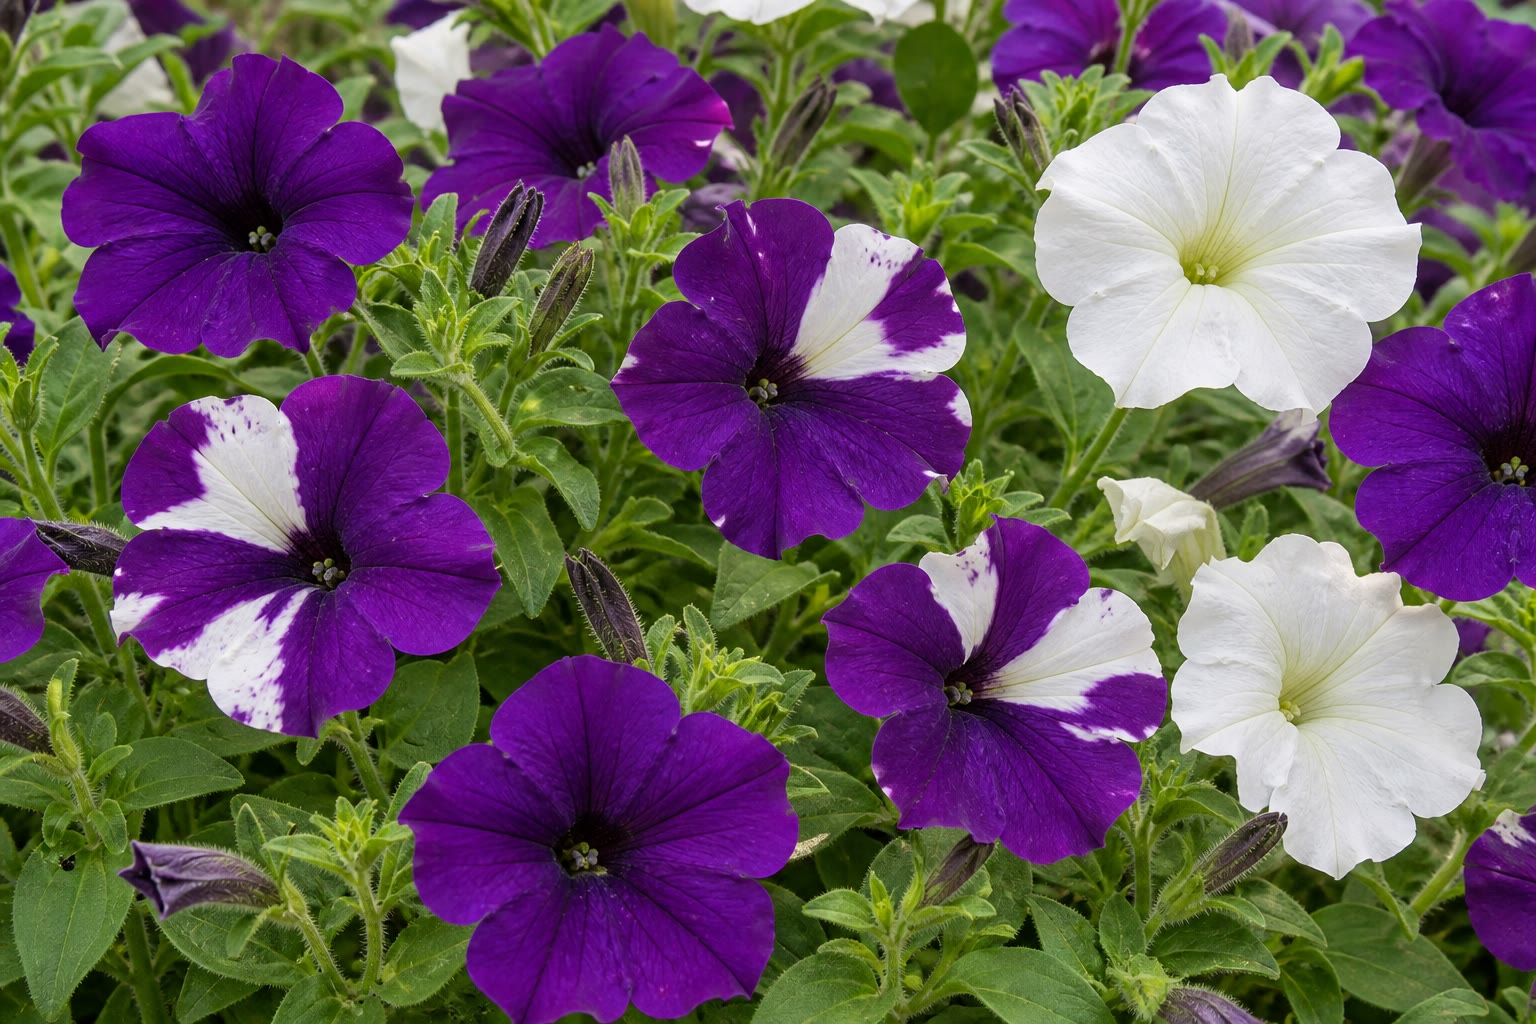
\includegraphics[width=0.46\linewidth]{images/book5/ai/b5-02-petunia-cosuppression.jpg}\hspace{0.04\linewidth}
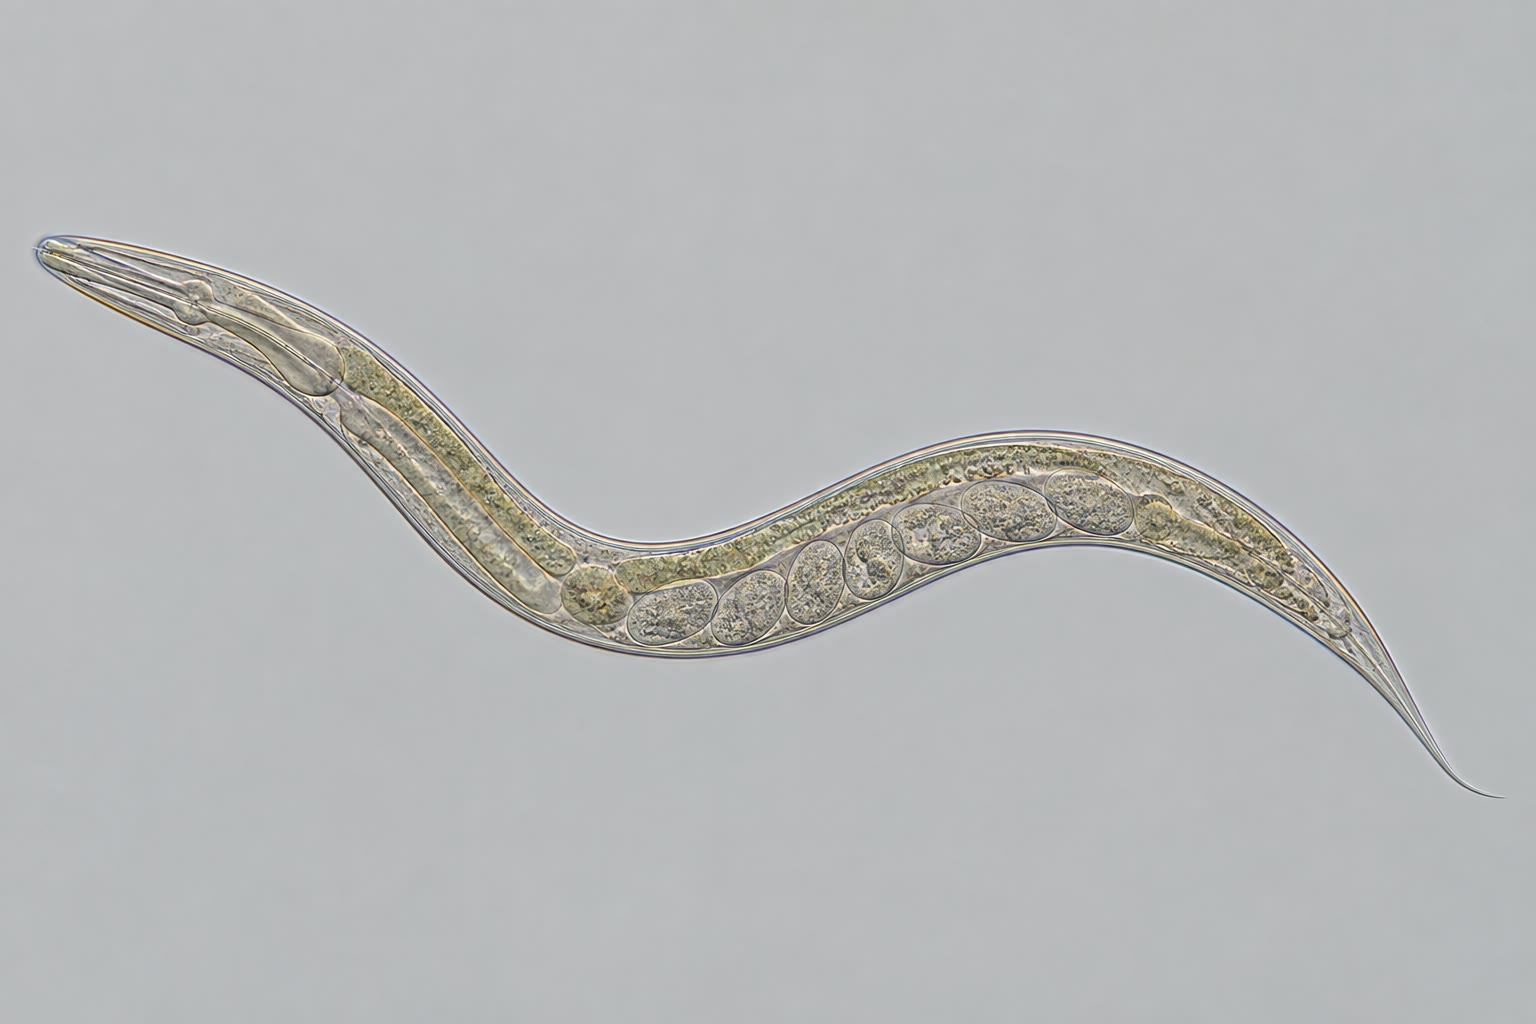
\includegraphics[width=0.46\linewidth]{images/book5/ai/b5-02-c-elegans.jpg}

{\small À esquerda: petúnias que carregam um gene extra de pigmento,
com os setores brancos da cossupressão. À direita: o nematódeo
\emph{Caenorhabditis elegans}, de cerca de um milímetro e
transparente, no qual o RNA de fita dupla injetado silenciou o gene
correspondente no animal inteiro e em sua prole.}
\end{omfigure}

\begin{definition}[MicroRNAs]\label{def:b3:rna-regulation:mirna}
\index{microRNA!biogênese}\index{Drosha}\index{sequência semente}
Um \emph{\omterm{def:b3:rna-regulation:ncrna}{microRNA}} é codificado no genoma --- num gene próprio ou num
íntron de um gene codificador de proteína --- e transcrito pela
RNA-polimerase II como um longo transcrito primário (pri-miRNA) que
contém um grampo de cerca de \qty{70}{nt}. No núcleo a RNase III
\emph{Drosha}, com sua parceira DGCR8, recorta o grampo (o pré-miRNA);
a exportina-5 o leva ao citoplasma, onde a \omterm{def:b3:rna-regulation:rnai}{Dicer} remove a alça,
deixando um dúplex de \qty{22}{nt}. Uma das fitas é carregada na
\omterm{def:b3:rna-regulation:rnai}{Argonauta}. O miRNA maduro reconhece seus alvos sobretudo por sua
\emph{semente}, os nucleotídeos 2 a 8, que pareia com sítios em geral
na região 3$'$ não traduzida de um mensageiro; o resto do miRNA pareia
de modo imperfeito, e por isso o alvo não é clivado, mas reprimido: o
\omterm{def:b3:rna-regulation:rnai}{RISC} recruta proteínas que encurtam a cauda poli(A), removem o
capuz e inibem a tradução, e o mensageiro é degradado mais depressa.
Como uma semente tem apenas sete nucleotídeos, um miRNA tem centenas
de alvos, e mais da metade dos genes humanos codificadores de proteína
carrega sítios conservados para ao menos um das várias centenas de
miRNAs humanos identificados com confiança.
\end{definition}

\begin{proof}[Evidência]
O \emph{lin-4}, um gene necessário para o verme passar de seu primeiro
estágio larval ao segundo, foi mostrado por Lee, Feinbaum e Ambros
(1993) codificar não uma proteína, mas um RNA de \qty{22}{nt},
complementar a sete sítios na região 3$'$ não traduzida do mensageiro
do \emph{lin-14}, o gene que ele reprimia. Quando a larva entra no
segundo estágio a proteína LIN-14 desaparece enquanto seu mRNA
permanece: a repressão é pós-transcricional. Reinhart e colaboradores
(2000) encontraram um segundo RNA desses, o \emph{let-7}, controlando
as transições larvais posteriores; Pasquinelli (2000) encontrou o
\emph{let-7} em moscas e em humanos, com a mesma sequência, o que fez
de uma curiosidade de verme um mecanismo geral.
\end{proof}

\begin{omfigure}
\begin{tikzpicture}[every node/.style={font=\scriptsize}, >=stealth]
  % nucleus box
  \draw[rounded corners=8pt, thick, gray!60, fill=gray!6] (-0.4,-1.1) rectangle (5.2,2.7);
  \node[gray, anchor=south west] at (-0.3,-1.05) {núcleo};
  % gene and pri-miRNA
  \draw[very thick, omDef] (0,2.0) -- (2.4,2.0); \node[above] at (1.2,2.05) {gene de miRNA, Pol II};
  \draw[->, thick] (1.2,1.85) -- (1.2,1.35);
  % hairpin
  \draw[thick, omThm!70!black] (0.2,1.0) -- (0.9,1.0) .. controls (1.0,1.0) and (1.05,0.9) .. (1.1,0.5) .. controls (1.15,0.1) and (1.25,0.1) .. (1.3,0.5) .. controls (1.35,0.9) and (1.4,1.0) .. (1.5,1.0) -- (2.2,1.0);
  \draw[thick, omThm!70!black] (1.1,0.5) -- (1.3,0.5);
  \node[below] at (1.2,0.0) {grampo do pri-miRNA};
  % Drosha
  \draw[thick, fill=omExo!35] (2.9,0.7) ellipse (0.55 and 0.28); \node at (2.9,0.7) {Drosha};
  \draw[->, thick] (2.3,0.85) -- (2.4,0.75);
  \draw[->, thick] (3.5,0.7) -- (4.2,0.7) node[midway, above] {corte};
  % pré-miRNA
  \draw[thick, omThm!70!black] (4.3,0.9) .. controls (4.5,0.9) and (4.55,0.4) .. (4.6,0.1) .. controls (4.65,-0.2) and (4.75,-0.2) .. (4.8,0.1) .. controls (4.85,0.4) and (4.9,0.9) .. (5.1,0.9);
  \node[below, align=center] at (4.7,-0.25) {pré-miRNA\\\qty{70}{nt}};
  % export
  \draw[->, thick] (5.35,0.4) -- (6.3,0.4) node[midway, above, xshift=0.2cm] {exportina-5};
  % cytoplasm
  \node[gray, anchor=north west] at (5.5,2.65) {citoplasma};
  \draw[thick, fill=omExo!35] (6.9,0.4) ellipse (0.5 and 0.28); \node at (6.9,0.4) {Dicer};
  \draw[->, thick] (7.45,0.4) -- (8.1,0.4);
  \draw[thick, omThm!70!black] (8.2,0.55) -- (9.6,0.55); \draw[thick, omThm!70!black] (8.35,0.25) -- (9.75,0.25);
  \node[below, align=center] at (8.95,0.15) {dúplex de \qty{22}{nt}};
  \draw[->, thick] (8.95,-0.4) -- (8.95,-0.9) node[midway, right] {uma fita é carregada};
  % RISC on mRNA
  \draw[thick, fill=omProp!35] (8.95,-1.45) ellipse (0.85 and 0.35); \node at (8.95,-1.45) {Argonauta};
  \draw[thick, omThm!70!black] (8.3,-1.85) -- (9.6,-1.85);
  \draw[very thick, omDef] (5.6,-2.15) -- (11.4,-2.15);
  \node[below] at (6.4,-2.2) {mRNA: região codificadora}; \node[below] at (10.3,-2.2) {3$'$ UTR, sítio-alvo};
  \draw[omDef, thick] (11.4,-2.15) -- (11.8,-2.15) node[right] {AAAA};
  \draw[->, thick, omThm] (9.9,-1.5) -- (10.9,-1.5) node[right, align=left] {desadenilação,\\degradação, menos\\tradução};
  \node[below, align=center] at (8.95,-2.7) {a semente (nt 2--8)\\pareia com o sítio};
\end{tikzpicture}

{\small Biogênese de um \omterm{def:b3:rna-regulation:ncrna}{microRNA}. O grampo é recortado do transcrito
primário pela \omterm{def:b3:rna-regulation:mirna}{Drosha} no núcleo, exportado, aparado pela \omterm{def:b3:rna-regulation:rnai}{Dicer} até um
dúplex de \qty{22}{nt}, e uma das fitas é carregada na \omterm{def:b3:rna-regulation:rnai}{Argonauta}. A
semente pareia com um sítio na região 3$'$ não traduzida de um
mensageiro, e o mensageiro é desadenilado, degradado e menos
traduzido.}
\end{omfigure}

\begin{theorem}[O que um microRNA faz ao nível e à velocidade de um mensageiro]\label{thm:b3:rna-regulation:mirna-kinetics}
\index{meia-vida do mRNA}\index{tempo de resposta}
Um mensageiro é sintetizado a uma taxa constante $k$ e degradado com
taxa de primeira ordem $\gamma$; um \omterm{def:b3:rna-regulation:ncrna}{microRNA} presente no nível $R$
acrescenta um termo de decaimento $\gamma' R\, m$. Então o nível de
mRNA $m(t)$ obedece a
\[
\frac{\mathrm{d}m}{\mathrm{d}t} = k - (\gamma + \gamma' R)\, m,
\qquad
m^{*} = \frac{k}{\gamma + \gamma' R},
\qquad
m(t) = m^{*} + (m_{0} - m^{*})\,e^{-(\gamma + \gamma' R)t}.
\]
O \omterm{def:b3:rna-regulation:ncrna}{microRNA} baixa o estado estacionário pelo fator $1 + \gamma' R/
\gamma$ e encurta a constante de tempo de toda mudança em $m$ de
$1/\gamma$ para $1/(\gamma + \gamma' R)$ pelo mesmo fator. Um gene
regulado por \omterm{def:b3:rna-regulation:ncrna}{microRNA} é, portanto, ao mesmo tempo mais silencioso e
mais rápido: alcança antes um novo estado estacionário depois que seu
promotor muda, e as flutuações de sua transcrição são amortecidas.
\end{theorem}
\begin{proof}
A equação é linear com coeficientes constantes; seu ponto fixo é
$m^{*}$, onde o lado direito se anula, e escrever $u = m - m^{*}$ dá
$\mathrm{d}u/\mathrm{d}t = -(\gamma + \gamma' R)\,u$, de onde vem a
exponencial. O tempo de meia-resposta da aproximação é $\ln 2/(\gamma + \gamma'
R)$, e $\gamma = \ln 2 / t_{1/2}$, em que $t_{1/2}$ é a meia-vida
natural do mensageiro.
\end{proof}

\begin{example}[Uma repressão de quatro vezes]\label{ex:b3:rna-regulation:fourfold}
Um mensageiro com meia-vida natural de \qty{30}{min} ($\gamma =
\qty{0.023}{min^{-1}}$), transcrito a $k = 2$ moléculas por minuto,
assenta-se em $m^{*} = 2/0.023 \approx 87$ cópias por célula e leva
\qty{30}{min} para percorrer metade do caminho até um novo nível
depois que seu promotor muda. Um \omterm{def:b3:rna-regulation:ncrna}{microRNA} que triplica sua taxa de
decaimento ($\gamma' R = 3\gamma$) o leva a $22$ cópias e reduz o
tempo de meia-resposta a \qty{7.5}{min}. Os mesmos números, lidos ao
contrário, mostram por que os nocautes de miRNA muitas vezes têm
fenótipos brandos: uma mudança de quatro vezes num mensageiro que já é
tamponado adiante pode deixar o organismo quase normal, e o efeito
aparece sob estresse ou no cronograma.
\end{example}

\begin{omfigure}
\begin{tikzpicture}
\begin{axis}[
  width=0.7\linewidth, height=5.6cm,
  axis x line=bottom, axis y line=left,
  xmin=0, xmax=120, ymin=0, ymax=100,
  xlabel={tempo após o promotor ligar (min)}, ylabel={mRNA por célula},
  xlabel style={font=\small, at={(axis description cs:0.5,-0.12)}, anchor=north},
  ylabel style={font=\small},
  tick label style={font=\small}, xtick={0,30,60,90,120}, ytick={0,22,50,87},
  clip=false,
]
\addplot[very thick, omDef, domain=0:120, samples=80] {87*(1-exp(-0.0231*x))};
\addplot[very thick, omThm, domain=0:120, samples=80] {21.7*(1-exp(-0.0924*x))};
\addplot[dashed, gray, domain=0:120, samples=2] {87};
\addplot[dashed, gray, domain=0:120, samples=2] {21.7};
\node[font=\scriptsize, omDef, anchor=south west] at (axis cs:5,90) {sem microRNA: $m^{*} = 87$, meia-resposta \qty{30}{min}};
\node[font=\scriptsize, omThm, anchor=south west] at (axis cs:40,24) {com microRNA, $\gamma' R = 3\gamma$: $m^{*} = 22$, meia-resposta \qty{7.5}{min}};
\end{axis}
\end{tikzpicture}

{\small Subida de um mensageiro depois que seu promotor é ligado, com
os números do \cref{ex:b3:rna-regulation:fourfold}. O \omterm{def:b3:rna-regulation:ncrna}{microRNA} baixa o
patamar quatro vezes e o alcança quatro vezes mais cedo.}
\end{omfigure}

\begin{method}[Silenciar um gene por RNAi]\label{met:b3:rna-regulation:knockdown}
\index{knockdown}\index{shRNA}
Para silenciar um gene sem tocar em seu DNA: (1) escolha uma sequência
de \qty{21}{nt} exclusiva de seu mensageiro, evitando correspondências
de semente com outros genes; (2) entregue-a como um dúplex sintético
de \omterm{def:b3:rna-regulation:ncrna}{siRNA} (transitório, alguns dias) ou como um RNA em grampo curto
(shRNA) expresso a partir de um vetor, que a \omterm{def:b3:rna-regulation:rnai}{Dicer} processa
continuamente; em vermes, alimente os animais com bactérias que
expressam o RNA de fita dupla; (3) meça o mensageiro por PCR
quantitativa e a proteína por imunotransferência, esperando uma perda
de \qtyrange{70}{95}{\%} em vez da ausência completa de um nocaute;
(4) controle os efeitos fora do alvo com um segundo \omterm{def:b3:rna-regulation:ncrna}{siRNA} que não se
sobreponha ao primeiro e com um resgate por uma versão do gene
resistente ao RNAi. Um knockdown é uma perda de função parcial e
reversível; as terapias gênicas hoje aprovadas com esse princípio
entregam \omterm{def:b3:rna-regulation:ncrna}{siRNAs} contra mensageiros hepáticos (transtirretina, PCSK9)
acoplados a um açúcar que o hepatócito capta.
\end{method}

\section{RNAs pequenos que guardam o genoma}

\begin{definition}[piRNAs e silenciamento de transpósons]\label{def:b3:rna-regulation:pirna}
\index{piRNA!pingue-pongue}\index{silenciamento de transpósons}\index{disgenesia híbrida}
Os \emph{\omterm{def:b3:rna-regulation:ncrna}{piRNAs}} são RNAs de \numrange{26}{31} nucleotídeos, feitos sem
a \omterm{def:b3:rna-regulation:rnai}{Dicer} a partir de longos transcritos de fita simples de
\emph{agrupamentos de \omterm{def:b3:rna-regulation:ncrna}{piRNA}} genômicos --- cemitérios de cópias
defeituosas de transpósons --- e carregados na subfamília PIWI das
proteínas \omterm{def:b3:rna-regulation:rnai}{Argonauta} na linhagem germinativa. Um \omterm{def:b3:rna-regulation:ncrna}{piRNA} antissenso a um
transpóson guia a clivagem dos transcritos desse transpóson; o
fragmento clivado se torna um novo \omterm{def:b3:rna-regulation:ncrna}{piRNA} senso, que por sua vez corta
transcritos do agrupamento para fazer mais \omterm{def:b3:rna-regulation:ncrna}{piRNAs} antissenso --- o
ciclo \emph{pingue-pongue}, uma amplificação que mira justamente o
transpóson que estiver ativo. Proteínas PIWI nucleares também dirigem
a metilação da H3K9 e a \omterm{def:b3:chromatin-epigenetics:methylation}{metilação do DNA} às cópias genômicas do
transpóson, ligando o RNA às marcas de \omterm{def:b3:chromatin-epigenetics:nucleosome}{cromatina} do
\cref{ch:b3:chromatin-epigenetics}. A mãe deposita seus \omterm{def:b3:rna-regulation:ncrna}{piRNAs} no
óvulo; uma fêmea cuja linhagem nunca encontrou um transpóson não tem
\omterm{def:b3:rna-regulation:ncrna}{piRNAs} contra ele, e sua prole com um macho que o carrega é estéril
--- a \emph{disgenesia híbrida}, vista primeiro em cruzamentos de
\emph{Drosophila} entre linhagens de laboratório e selvagens.
\end{definition}

\begin{proposition}[Silenciamento da cromatina dirigido por RNA]\label{prop:b3:rna-regulation:rddm}
\index{metilação do DNA dirigida por RNA}
Nas plantas, uma via dedicada --- a RNA-polimerase IV transcreve um
loco, uma RNA-polimerase dependente de RNA o torna de fita dupla, uma
\omterm{def:b3:rna-regulation:rnai}{Dicer} corta \omterm{def:b3:rna-regulation:ncrna}{siRNAs} de \qty{24}{nt}, a \omterm{def:b3:rna-regulation:rnai}{Argonauta}~4 os leva de volta aos
transcritos nascentes da polimerase V no mesmo loco e recruta a
metiltransferase DRM2 --- metila o DNA de transpósons e de sequências
repetidas; é o mecanismo da paramutação. Na levedura de fissão,
\omterm{def:b3:rna-regulation:ncrna}{siRNAs} das repetições centroméricas recrutam a metiltransferase da
H3K9 e constroem a \omterm{def:b3:chromatin-epigenetics:nucleosome}{heterocromatina} de que o centrômero precisa. Nos
dois casos um RNA encontra um lugar no genoma por complementaridade e
ali se escreve uma marca de \omterm{def:b3:chromatin-epigenetics:nucleosome}{cromatina}: sequência-específica,
autorreforçadora e hereditária ao longo das divisões.
\end{proposition}

\section{A vida de um mensageiro}

\begin{definition}[Splicing regulado]\label{def:b3:rna-regulation:splicing}
\index{splicing alternativo!regulação}\index{proteína SR}\index{hnRNP}\index{salto de éxon}
O splicing alternativo produz mensageiros diferentes a partir de um só
gene pelo \emph{salto de éxon}, pela escolha entre éxons mutuamente
exclusivos, pela retenção de um íntron ou pelo uso de sítios de
splicing 5$'$ ou 3$'$ alternativos. Ele é regulado por proteínas
ligadoras de RNA que se ligam a elementos de sequência nos éxons e
íntrons próximos de um sítio de splicing: as \emph{proteínas SR}
ligadas a intensificadores exônicos recrutam o spliceossomo e promovem
a inclusão do éxon, as proteínas \emph{hnRNP} ligadas a silenciadores
a bloqueiam, e o desfecho numa dada célula é fixado pelas quantidades
relativas dos dois tipos. Mais de \qty{90}{\%} dos genes humanos com
vários éxons sofrem splicing alternativo; o gene \emph{Dscam} de
\emph{Drosophila}, com quatro blocos de éxons mutuamente exclusivos
(12, 48, 33 e 2 alternativas), pode produzir \num{38016} proteínas
distintas, cada neurônio expressando um conjunto diferente que permite
a seus ramos reconhecer-se e evitar-se mutuamente.
\end{definition}

\begin{proof}[Evidência]
O sexo de uma mosca-das-frutas é decidido por uma cascata de splicing.
Nas fêmeas o gene \emph{Sex-lethal} (\emph{Sxl}) produz uma proteína
funcional; a SXL é uma proteína ligadora de RNA que bloqueia um sítio
de splicing em seu próprio transcrito (de modo que um éxon com códon
de parada é saltado e a proteína continua sendo feita) e no transcrito
do \emph{transformer}, forçando o splicing feminino; a TRA, junto com
a TRA-2, liga-se então a um intensificador exônico no transcrito do
\emph{doublesex} e dirige a forma feminina do fator de transcrição
DSX. Nos machos, sem SXL, cada um desses transcritos toma o splicing
padrão, o \emph{transformer} contém um códon de parada, e a DSX sai na
forma masculina. Toda característica sexualmente dimórfica da mosca
decorre de qual DSX é feita; uma fêmea com \emph{tra} mutado
desenvolve-se como macho.
\end{proof}

\begin{definition}[Estabilidade e localização do mRNA]\label{def:b3:rna-regulation:stability}
\index{elemento rico em AU}\index{localização do mRNA}\index{elemento responsivo ao ferro}
A \emph{meia-vida} de um mensageiro vai de minutos a dias e é fixada
por elementos de sua região 3$'$ não traduzida. Os \emph{elementos
ricos em AU} (repetições AUUUA) nos mensageiros de citocinas, fatores
de crescimento e proto-oncogenes são ligados por proteínas que
recrutam desadenilases e dão meias-vidas de \qtyrange{10}{30}{min}, de
modo que uma rajada de transcrição produz uma rajada de proteína e
nada mais; mutações que os removem causam superexpressão e, para
alguns proto-oncogenes, câncer. Os \emph{elementos de localização},
muitas vezes estruturados, são ligados por adaptadores que ligam o
mensageiro a um motor: os mensageiros de \emph{bicoid} e de
\emph{oskar} são levados aos dois polos do óvulo da mosca pela dineína
e pela cinesina sobre microtúbulos, o mensageiro da $\beta$-actina
à borda de avanço de um fibroblasto, e os mensageiros de proteínas
sinápticas para dentro dos dendritos, onde são traduzidos sob demanda.
O \emph{elemento responsivo ao ferro} (IRE), uma haste--alça ligada
pelas proteínas reguladoras de ferro IRP1 e IRP2 quando o ferro é
escasso, faz dois trabalhos opostos a partir de duas posições: na
região 5$'$ não traduzida do mensageiro da ferritina, a IRP ligada
bloqueia o ribossomo; na região 3$'$ não traduzida do mensageiro do
receptor de transferrina, a IRP ligada protege o transcrito de uma
nuclease.
\end{definition}

\begin{example}[O ferro, lido por um grampo]\label{ex:b3:rna-regulation:iron}
Quando o ferro está baixo, a IRP liga os dois mensageiros: a ferritina,
a proteína de armazenamento, não é traduzida, e o receptor de
transferrina, que importa ferro, é estabilizado e abundante --- a
célula armazena menos e importa mais. Quando o ferro está alto, ele
converte a IRP1 numa aconitase (ela adquire um agrupamento
ferro--enxofre e perde sua afinidade por RNA) e dispara a degradação da
IRP2: a ferritina é traduzida, o mensageiro do receptor decai em
minutos, e a célula armazena mais e importa menos. Nenhuma mudança de
transcrição é necessária. Uma mutação pontual no IRE da ferritina que
impede a ligação da IRP causa síntese constitutiva de ferritina e a
síndrome hereditária hiperferritinemia--catarata.
\end{example}

\begin{omfigure}
\begin{tikzpicture}[every node/.style={font=\scriptsize}, >=stealth]
  \foreach \yy/\state in {2.2/pouco ferro, -0.9/muito ferro} {
    \node[left, font=\small\bfseries] at (-0.2,\yy+0.35) {\state};
    % ferritin mRNA
    \draw[very thick, omDef] (0.3,\yy+0.6) -- (4.6,\yy+0.6); \node[below] at (3.3,\yy+0.4) {mRNA da ferritina};
    \draw[thick, omThm!70!black] (0.9,\yy+0.6) .. controls (0.9,\yy+1.15) and (1.3,\yy+1.15) .. (1.3,\yy+0.6); \node[below] at (1.1,\yy+0.55) {IRE};
    \draw[fill=omDef!20, thick] (2.2,\yy+0.42) rectangle (4.4,\yy+0.78);
    % TfR mRNA
    \draw[very thick, omDef] (6.2,\yy+0.6) -- (10.6,\yy+0.6); \node[below, font=\tiny] at (7.1,\yy+0.4) {mRNA do receptor de transferrina};
    \draw[fill=omDef!20, thick] (6.4,\yy+0.42) rectangle (8.6,\yy+0.78);
    \foreach \x in {9.0,9.5,10.0} \draw[thick, omThm!70!black] (\x,\yy+0.6) .. controls (\x,\yy+1.1) and (\x+0.35,\yy+1.1) .. (\x+0.35,\yy+0.6);
    \node[below, font=\tiny] at (9.9,\yy+0.55) {IREs (3$'$ UTR)};
  }
  % low iron: IRP bound
  \draw[thick, fill=omProp!40] (1.1,3.35) ellipse (0.4 and 0.24); \node at (1.1,3.35) {IRP};
  \node[right, omThm] at (1.55,3.35) {ribossomo bloqueado: sem ferritina};
  \foreach \x in {9.18,9.68,10.18} { \draw[thick, fill=omProp!40] (\x,3.35) ellipse (0.28 and 0.2); }
  \node[above, omMeth!70!black] at (9.7,3.75) {protegido da nuclease: receptor estável e abundante};
  \node[below, omMeth!70!black] at (1.1,1.75) {armazena menos};
  \node[below, omMeth!70!black] at (7.4,1.75) {importa mais};
  % high iron: IRP off
  \node[right, omMeth!70!black] at (1.55,0.25) {traduzido: ferritina produzida};
  \node[right, omThm, align=left] at (10.7,-0.3) {nuclease:\\o mRNA decai};
  \node[below, omThm] at (1.1,-1.35) {armazena mais};
  \node[below, omThm] at (7.4,-1.35) {importa menos};
\end{tikzpicture}

{\small O \omterm{def:b3:rna-regulation:stability}{elemento responsivo ao ferro}. Com pouco ferro a proteína
reguladora de ferro liga os grampos IRE: na extremidade 5$'$ do
mensageiro da ferritina ela bloqueia a tradução, na extremidade 3$'$ do
mensageiro do receptor de transferrina ela bloqueia uma nuclease. Com
muito ferro a proteína solta os dois: a ferritina é feita, o mensageiro
do receptor decai.}
\end{omfigure}

\begin{proposition}[Controle traducional]\label{prop:b3:rna-regulation:translation}
\index{controle traducional}\index{eIF2}\index{ribosswitch}\index{fase de leitura aberta a montante}
A etapa de iniciação é o ponto usual de controle da tradução. A
fosforilação do fator de iniciação \emph{eIF2} por cinases que
percebem a privação de aminoácidos, proteínas mal enoveladas, RNA
viral de fita dupla ou deficiência de heme desliga a iniciação geral
em minutos, poupando alguns poucos mensageiros com características
especiais --- em particular os que têm \emph{\omterm{prop:b3:rna-regulation:translation}{fases de leitura aberta a
montante}}, fases curtas na região 5$'$ não traduzida que normalmente
prendem ribossomos e que, sob estresse, são contornadas, de modo que
os fatores de resposta ao estresse (GCN4 na levedura, ATF4 nos
mamíferos) são feitos exatamente quando todo o resto não é. O fator de
ligação ao capuz eIF4E é mantido inativo por proteínas ligadoras de
4E até que a cinase de sinalização de crescimento mTOR as fosforile:
uma célula traduz a pleno regime só quando os nutrientes e os fatores
de crescimento o autorizam. Nas bactérias, os \emph{ribosswitches}
fazem isso sem proteína alguma: uma região 5$'$ estruturada liga um
metabólito (pirofosfato de tiamina, S-adenosilmetionina, uma purina)
e, ao ligá-lo, redobra-se para enterrar o sítio de ligação do
ribossomo ou para formar um terminador de transcrição, de modo que um
óperon biossintético se desliga quando seu produto é abundante.
\end{proposition}

\begin{omfigure}
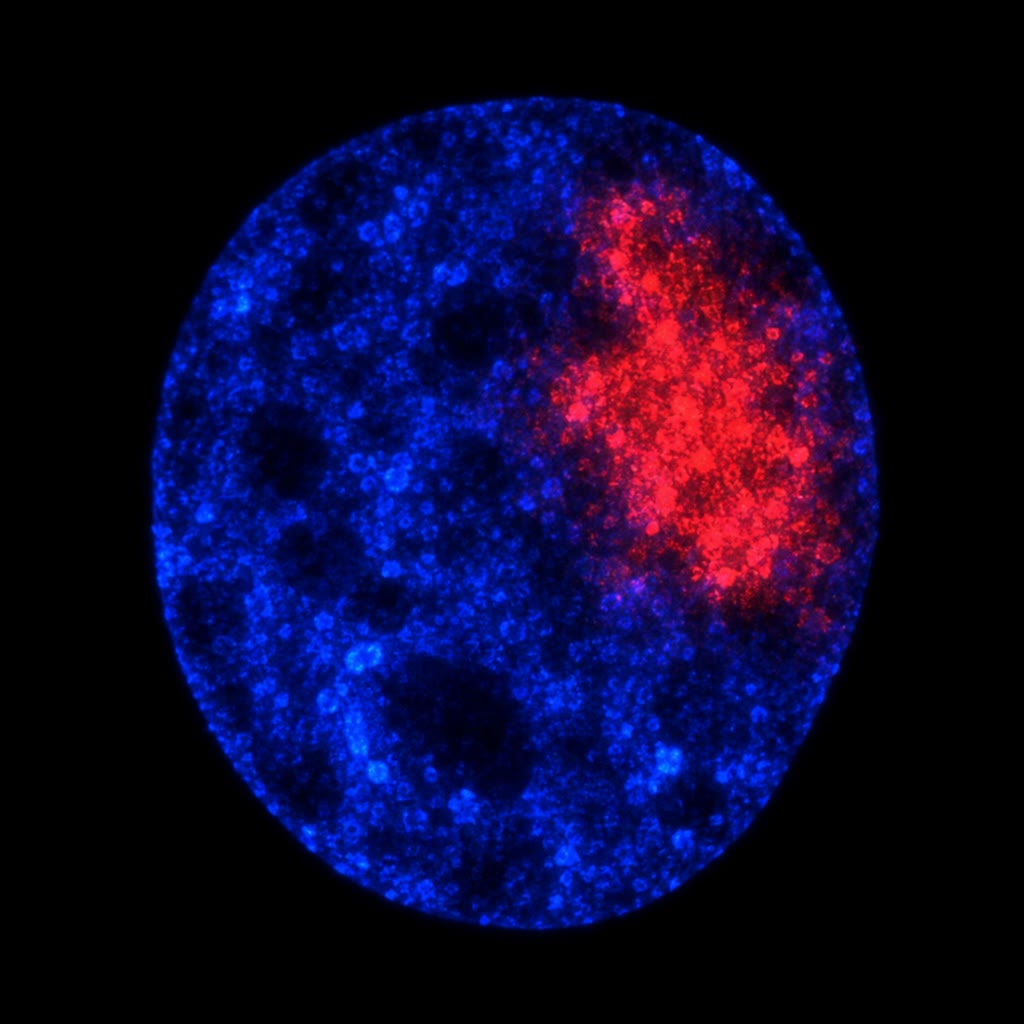
\includegraphics[width=0.36\linewidth]{images/book5/ai/b5-02-lncrna-nucleus.jpg}

{\small Um \omterm{def:b3:rna-regulation:ncrna}{RNA longo não codificante} em ação: o transcrito \emph{\omterm{def:b3:chromatin-epigenetics:x-inactivation}{Xist}}
(vermelho), detectado por hibridação fluorescente, recobre o território
de um cromossomo X num núcleo feminino (DNA em azul).}
\end{omfigure}

\begin{remark}[O que o controle pós-transcricional compra]\label{rem:b3:rna-regulation:why}
O controle transcricional age através do núcleo, com um atraso de
minutos a horas até que um novo mensageiro seja feito, exportado e
traduzido. O controle do próprio mensageiro age onde a proteína é
necessária, em segundos a minutos, e pode ser local: um único
dendrito traduzindo um mensageiro numa sinapse, a borda de avanço de
um fibroblasto produzindo actina onde ele rasteja. Ele também faz de
um gene muitas proteínas, e deixa um só sinal --- o ferro, um
aminoácido, um \omterm{def:b3:rna-regulation:ncrna}{microRNA} --- coordenar centenas de mensageiros ao mesmo
tempo sem tocar num único promotor.
\end{remark}

\section{Exercícios}

\begin{exercise}[$\star$]\label{exo:b3:rna-regulation:1}
Distinga miRNA, \omterm{def:b3:rna-regulation:ncrna}{siRNA} e \omterm{def:b3:rna-regulation:ncrna}{piRNA} quanto à origem, ao comprimento, à
dependência da \omterm{def:b3:rna-regulation:rnai}{Dicer} e ao que fazem a seus alvos.
\end{exercise}

\begin{exercise}[$\star$]\label{exo:b3:rna-regulation:2}
Trace a biogênese de um \omterm{def:b3:rna-regulation:ncrna}{microRNA} desde seu gene até um mensageiro
reprimido, nomeando a enzima de cada corte.
\end{exercise}

\begin{exercise}[$\star$]\label{exo:b3:rna-regulation:3}
Por que injetar RNA senso de \emph{unc-22} em vermes silenciava o gene
nos primeiros experimentos, e o que Fire e Mello mudaram?
\end{exercise}

\begin{exercise}[$\star$]\label{exo:b3:rna-regulation:4}
O que acontece com a ferritina e com o receptor de transferrina quando
uma célula é privada de ferro? Qual etapa da expressão é controlada em
cada caso?
\end{exercise}

\begin{exercise}[$\star\star$]\label{exo:b3:rna-regulation:5}
Um mensageiro tem meia-vida de \qty{2}{h} e é feito a $5$ moléculas
por minuto. Calcule seu nível estacionário e, em seguida, o nível e o
tempo de meia-resposta quando um \omterm{def:b3:rna-regulation:ncrna}{microRNA} dobra sua taxa de
decaimento.
\end{exercise}

\begin{exercise}[$\star\star$]\label{exo:b3:rna-regulation:6}
Uma semente de sete nucleotídeos corresponde a uma sequência aleatória
com probabilidade $4^{-7}$. Num conjunto de \num{20000} mensageiros
com regiões 3$'$ não traduzidas de \qty{1000}{nt} em média, quantos
sítios uma semente de \omterm{def:b3:rna-regulation:ncrna}{microRNA} corresponde por acaso? O que, então,
distingue um alvo real?
\end{exercise}

\begin{exercise}[$\star\star$]\label{exo:b3:rna-regulation:7}
Preveja o sexo de uma mosca (a) com uma mutação de perda de função de
\emph{tra} e dois cromossomos X; (b) que expressa TRA a partir de um
transgene constitutivo, com um X; (c) desprovida de \emph{dsx}.
\end{exercise}

\begin{exercise}[$\star\star$]\label{exo:b3:rna-regulation:8}
O mensageiro de um proto-oncogene tem normalmente meia-vida de
\qty{15}{min} por causa de um \omterm{def:b3:rna-regulation:stability}{elemento rico em AU}. Uma translocação
cromossômica remove o elemento e a meia-vida passa a \qty{3}{h}. Por
qual fator sobe o nível da proteína, se a tradução e a degradação
proteica não mudam? Por que isso é oncogênico embora a proteína seja
normal?
\end{exercise}

\begin{exercise}[$\star\star$]\label{exo:b3:rna-regulation:9}
Uma linhagem de laboratório de \emph{Drosophila} não tem elementos P;
uma linhagem selvagem os carrega. Preveja a fertilidade da prole de
(a) fêmeas de laboratório $\times$ machos selvagens, (b) fêmeas
selvagens $\times$ machos de laboratório, e explique a assimetria com
os \omterm{def:b3:rna-regulation:ncrna}{piRNAs}.
\end{exercise}

\begin{exercise}[$\star\star\star$]\label{exo:b3:rna-regulation:10}
Usando o \cref{thm:b3:rna-regulation:mirna-kinetics}, argumente que a
proteína feita a partir de um mensageiro flutua menos, em termos
relativos, quando o mensageiro está sob controle de \omterm{def:b3:rna-regulation:ncrna}{microRNA}, para um
mesmo nível médio de mensageiro. (A proteína faz a média do mensageiro
ao longo de sua própria vida, e o mensageiro se renova mais depressa.)
Por que uma célula pagaria por um \omterm{def:b3:rna-regulation:ncrna}{microRNA} e por uma taxa de
transcrição maior para obter a mesma média?
\end{exercise}

\begin{exercise}[$\star\star\star$]\label{exo:b3:rna-regulation:11}
Nos vermes, uma RNA-polimerase dependente de RNA faz \omterm{def:b3:rna-regulation:ncrna}{siRNAs}
secundários a partir do mensageiro-alvo; nos mamíferos não há nenhuma.
Preveja, para cada um, se o silenciamento por uma única injeção de RNA
de fita dupla dura por muitas divisões celulares e se ele se espalha a
outros tecidos, e explique a consequência médica para os fármacos de
\omterm{def:b3:rna-regulation:ncrna}{siRNA}.
\end{exercise}

\begin{exercise}[$\star\star\star$]\label{exo:b3:rna-regulation:12}
Um lncRNA recém-anotado é expresso no coração. Planeje os experimentos
que distinguiriam (a) um RNA funcional, (b) um ato de transcrição
funcional cujo RNA é irrelevante e (c) ruído, e diga que resultado
cada um prevê.
\end{exercise}

\section{Problema: o cronômetro de um verme}

\begin{problem}[{Problema de fim de semana --- o interruptor
\emph{lin-4}/\emph{lin-14} do verme cronometrado com a cinética do
mensageiro, um RNA injetado diluído pelas divisões de um embrião e
resgatado por amplificação, o regulão do ferro quantificado e uma
contagem de splicing, terminando no fator de repressão, no tempo de
meia-resposta do interruptor e no número de divisões que um sinal não
amplificado sobrevive}]
\label{pb:b3:rna-regulation:1}
Dados: o mensageiro \emph{lin-14} é feito a $k = 3$ moléculas por
minuto por célula e tem meia-vida de \qty{40}{min}. A proteína LIN-14 é
feita a $\beta = 2$ por mensageiro por minuto e tem meia-vida de
\qty{3}{h}. A partir do início do segundo estágio larval, o RNA
\emph{lin-4} se acumula e acrescenta um termo de decaimento
$\gamma' R = 3\gamma$ ao mensageiro e, ao bloquear a iniciação,
reduz $\beta$ à metade. Um embrião de verme desenvolve-se de uma
célula a cerca de \num{550} células ao eclodir; um adulto tem
\num{959} células somáticas.

\medskip
\noindent\textbf{Parte I --- O mensageiro.}
\begin{enumerate}
  \item Calcule $\gamma$ e o nível estacionário do mensageiro
        \emph{lin-14} antes de o \emph{lin-4} aparecer.
  \item Calcule a taxa de degradação da proteína e o nível
        estacionário da proteína LIN-14.
  \item Uma vez presente o \emph{lin-4}, calcule o novo nível do
        mensageiro e a nova constante de tempo do mensageiro.
  \item Calcule o novo estado estacionário da proteína e o fator de
        repressão total sobre a proteína.
  \item Quanto tempo depois de o \emph{lin-4} aparecer o mensageiro
        chega à metade do caminho até seu novo nível? E a proteína ---
        que etapa limita a velocidade do interruptor?
  \item Os experimentos originais encontraram a proteína desaparecida
        enquanto o mRNA ainda era detectável. Isso é coerente com seus
        números? Que fração do mensageiro permanece?
\end{enumerate}

\medskip
\noindent\textbf{Parte II --- Diluição e amplificação.}
\begin{enumerate}[resume]
  \item A gônada de um verme recebe a injeção de $10^{6}$ moléculas de
        RNA de fita dupla, repartidas igualmente entre \num{250}
        óvulos. Quantas moléculas por óvulo?
  \item Se as moléculas fossem simplesmente repartidas a cada divisão,
        quantas teria cada célula da larva de \num{550} células ao
        eclodir? Após quantas divisões a mais a média cairia abaixo de
        uma por célula?
  \item Fire e Mello viram silenciamento no animal inteiro e em sua
        prole, com algumas moléculas por célula. Explique o que uma
        RNA-polimerase dependente de RNA acrescenta à explicação, e
        por que o efeito mesmo assim se desvanece após algumas
        gerações.
  \item Numa célula de mamífero sem essa polimerase, uma transfecção
        de \omterm{def:b3:rna-regulation:ncrna}{siRNA} põe \num{5000} dúplexes numa célula que se divide
        diariamente; o \omterm{def:b3:rna-regulation:rnai}{RISC} é estável, mas é diluído pela divisão.
        Após quantos dias a contagem cai abaixo de \num{100}, mais ou
        menos o número necessário para um silenciamento eficaz?
  \item Um \omterm{def:b3:rna-regulation:ncrna}{siRNA} terapêutico contra um mensageiro hepático é dado uma
        única vez e funciona por seis meses. Os hepatócitos raramente
        se dividem. Explique por que o mecanismo da questão 10 não o
        limita, e o que o limita.
  \item Uma semente de sete nucleotídeos corresponde ao acaso uma vez
        a cada $4^{7}$ nucleotídeos. O transcriptoma do verme tem
        cerca de \qty{20}{Mb} de sequência 3$'$ não traduzida. Quantas
        correspondências de semente ao acaso tem o \emph{lin-4}, e
        como os geneticistas souberam qual alvo importava?
\end{enumerate}

\medskip
\noindent\textbf{Parte III --- O regulão do ferro.}
\begin{enumerate}[resume]
  \item Em células ricas em ferro o mensageiro do receptor de
        transferrina tem meia-vida de \qty{10}{min}; com a IRP ligada,
        \qty{50}{min}. Sem mudança na transcrição, por qual fator sobe
        o mensageiro quando o ferro se torna escasso?
  \item O mensageiro da ferritina não muda de nível, mas sua tradução
        cai de $1$ para $0.05$ proteínas por mensageiro por minuto
        quando a IRP se liga. Por qual fator cai a síntese de
        ferritina?
  \item Combine os dois: por qual fator muda a razão entre capacidade
        de importação e capacidade de armazenamento entre os estados
        rico e pobre em ferro?
  \item A proteína IRP1 é ou uma proteína ligadora de RNA ou uma
        aconitase, conforme tenha ou não um agrupamento
        ferro--enxofre. Explique por que isso faz dela um sensor do
        próprio ferro, e não de um hormônio.
  \item Um paciente tem uma mutação no IRE da ferritina que abole a
        ligação da IRP. Preveja o nível de ferritina, o ferro sérico e
        por que o cristalino do olho é afetado.
  \item Explique numa frase por que o mesmo grampo pode ativar numa
        posição e reprimir em outra.
  \item A IRP2 não tem agrupamento ferro--enxofre; quando o ferro está
        alto ela é destruída por uma ubiquitina-ligase cuja própria
        estabilidade exige ferro e oxigênio. Por que uma célula
        manteria dois sensores de química tão diferente?
\end{enumerate}

\medskip
\noindent\textbf{Parte IV --- Contando isoformas.}
\begin{enumerate}[resume]
  \item O \emph{Dscam} tem blocos de éxons com 12, 48, 33 e 2
        alternativas mutuamente exclusivas. Quantas isoformas? Se cada
        neurônio expressa cerca de $50$ ao acaso, qual é a
        probabilidade de dois neurônios dados compartilharem ao
        menos uma? (Use $1 - (1 -
        50/N)^{50}$.)
  \item Por que um neurônio se beneficia de ter isoformas que seus
        vizinhos quase certamente não têm?
  \item Um gene com $n$ éxons-cassete, cada um incluído ou saltado de
        modo independente, dá quantos mensageiros? Quantos para
        $n = 10$? Por que o número real num dado tipo celular é em
        geral muito menor?
  \item Na mosca, por que uma fêmea com dois cromossomos X mas um
        alelo \emph{Sxl} nulo morre em vez de simplesmente se
        desenvolver como macho? (Considere o que mais o sistema de
        contagem do X controla: a \omterm{def:b3:chromatin-epigenetics:x-inactivation}{compensação de dose} dos genes
        ligados ao X.)
  \item A SXL promove o splicing produtivo de seu próprio transcrito.
        Explique por que isso faz da decisão sexual uma memória que
        persiste depois que o sinal de contagem do X, presente apenas
        no embrião inicial, desapareceu, e relacione isso com os
        interruptores autossustentados do
        \cref{ch:b3:chromatin-epigenetics}.
  \item Resuma o cronômetro: o fator de repressão sobre a proteína
        LIN-14 (questão~4), o tempo de meia-resposta do interruptor do
        mensageiro (questão~5) e o número de divisões que um sinal não
        amplificado sobrevive antes de cair abaixo de uma molécula por
        célula (questão~8).
\end{enumerate}
\end{problem}
